\section{Extracting \mt}
Extracting \mt consists of two main steps. Initially, a local orientation direction (represented as a unit vector) is computed at each grid location.
Next, we compute a coarse set of poly-cylinders called \mt which traverses the data constrained by the local orientation directions. Sec.~\ref{subsec:reliable_hessian} describes the procedure to generate Reliable Hessians. Sec.~\ref{subsec:mt_properties}  describes the \mt and their properties. Sec.~\ref{subsec:mt_generation} details the creation of \mt.
\subsection{Computing Reliable Hessians}\label{subsec:reliable_hessian} 
The objective of this step is to associate each grid location with a unit vector which represents the orientation in the local neighborhood and a real value [0,1] that represents a measure of reliability of the orientation calculated at the grid location. A reliability score of 0 would mean the local orientation is not credible. While a score of 1 means the vector captures the local orientation inherent in the data with a high confidence

The input to this stage is the original scalar data, which is a uniform lattice grid in $\mathbb{R}^3$. We approximate the local orientation  by eigenvalue analysis of the Hessian matrix applied locally to each voxel.
The Hessian matrix captures the second-order structures inherent in the intensity (scalar values at grid vertex) variations around each grid location.
The eigen decomposition of the Hessian matrix gives the eigenvectors which describe the local second-order structure, which represents the local curvature of the image. The eigenvector corresponding the smallest eigenvalue gives the direction along which the curvature is smallest. This direction also termed as the principal direction, coincides with the direction of the tubular structure. 


Frangi et al.~\cite{Frangi1998} introduced a process that searches for geometric structures which are tubular. They defined 
a ``vesselnes" criterion based on the geometric ratios of the second order ellipsoid given by the local Hessian matrix.
In order to determine reliable Hessians, we compute the \textit{same} metric. We include their work here for completeness and direct the reader to~\cite{Frangi1998} for details. Let $\lambda_{K}$ be the eigenvalue with the $K^{th}$ smallest magnitude. Here, $|{\lambda}_{1}| \leq| {\lambda}_{2}|\leq| {\lambda}_{3}| $ are the eigenvalues of the Hessian matrix. Specifically, a pixel belonging to a vessel region will have small $\lambda_{1}$ ($|\lambda_{1}|\approx 0$) and $\lambda_{2}$, $\lambda_{3}$ of large magnitude and of equal sign ($|\lambda_{1}| \ll |\lambda_{2}|$ and $|\lambda_{2}|\approx |\lambda_{3}|$). The sign indicates if the vessel is bright in a dark background or dark in a bright background. In our case the individual fibers are bright ($\lambda_2,\lambda_3 < 0$). The following measures are defined in~\cite{Frangi1998}.  
\begin{equation}\label{RA}
\mathcal{R_{A}}=\frac{\textrm{Largest  Cross Section}\big/ \pi}{{\textrm{Largest Axis Semi-length}}^{2}}=\frac{|\lambda_{2}|}{|\lambda_{3}|}
\end{equation}
\begin{equation}\label{RB}
\mathcal{R_{B}}=\frac{\textrm{Volume}\big/ (4\pi \big/ 3)}{{(\textrm{Largest Cross Section Area}\big/ \pi)}^{\frac{3}{2}}}=\frac{|\lambda_{1}|}{\sqrt{|\lambda_{2}\lambda_{3}|}}
\end{equation}
In Equation~\ref{RB}, $\mathcal{R_{B}}$ provides a measure of deviation from a blob like structure while in Equation~\ref{RA}, $\mathcal{R_{A}}$ distinguishes between plate-like and line-like structure. Grey-scale variations and close proximity of the fibers in our data make the Hessians computed at each voxels susceptible to errors. Thus, we compute reliable Hessians ($R_H$) to determine which locations in the volume provide reliable local orientation. 
$$
R_{H} = \left\{ \begin{array}{ccc}
0 & \mbox{ if $\lambda_{2}>0$ or $\lambda_{3}>0$} \\
(1-e^{\frac{\mathcal{-R_{A}}^{2}}{2\alpha^{2}}})
(e^{\frac{\mathcal{-R_{B}}^{2}}{2\beta^{2}}}) (1-e^{\frac{-s^2}{2c^2}}) &\mbox{ otherwise}
\end{array} \right.
$$
Variable $s$ is the Frobenius norm of the Hessian matrix. The value of $(1-e^{\frac{-s^2}{2c^2}})$ will be low in regions with no structure. The utility of the vesselness is a little different in our framework than Frangi et al.~\cite{Frangi1998}.
First, vesselness in biology is computed for different scales because the vessels can be of different sizes. In our case, usually the widths of individual fibers are known a priori.
Second, and more importantly, we do not have clear tubular structures embedded in a dark contrast matrix such as in blood vessels.
Instead, we are trying to associate each grid location  with a probable orientation based on its local second order structure. The $R_{H}$ is interpreted as a reliability measure of the local orientation.
Grid locations where the $R_{H}$ is above a cutoff threshold are marked as regions with reliable orientations (see Sec.~\ref{sec:param_choices}).

\begin{figure}[tb]
\centering
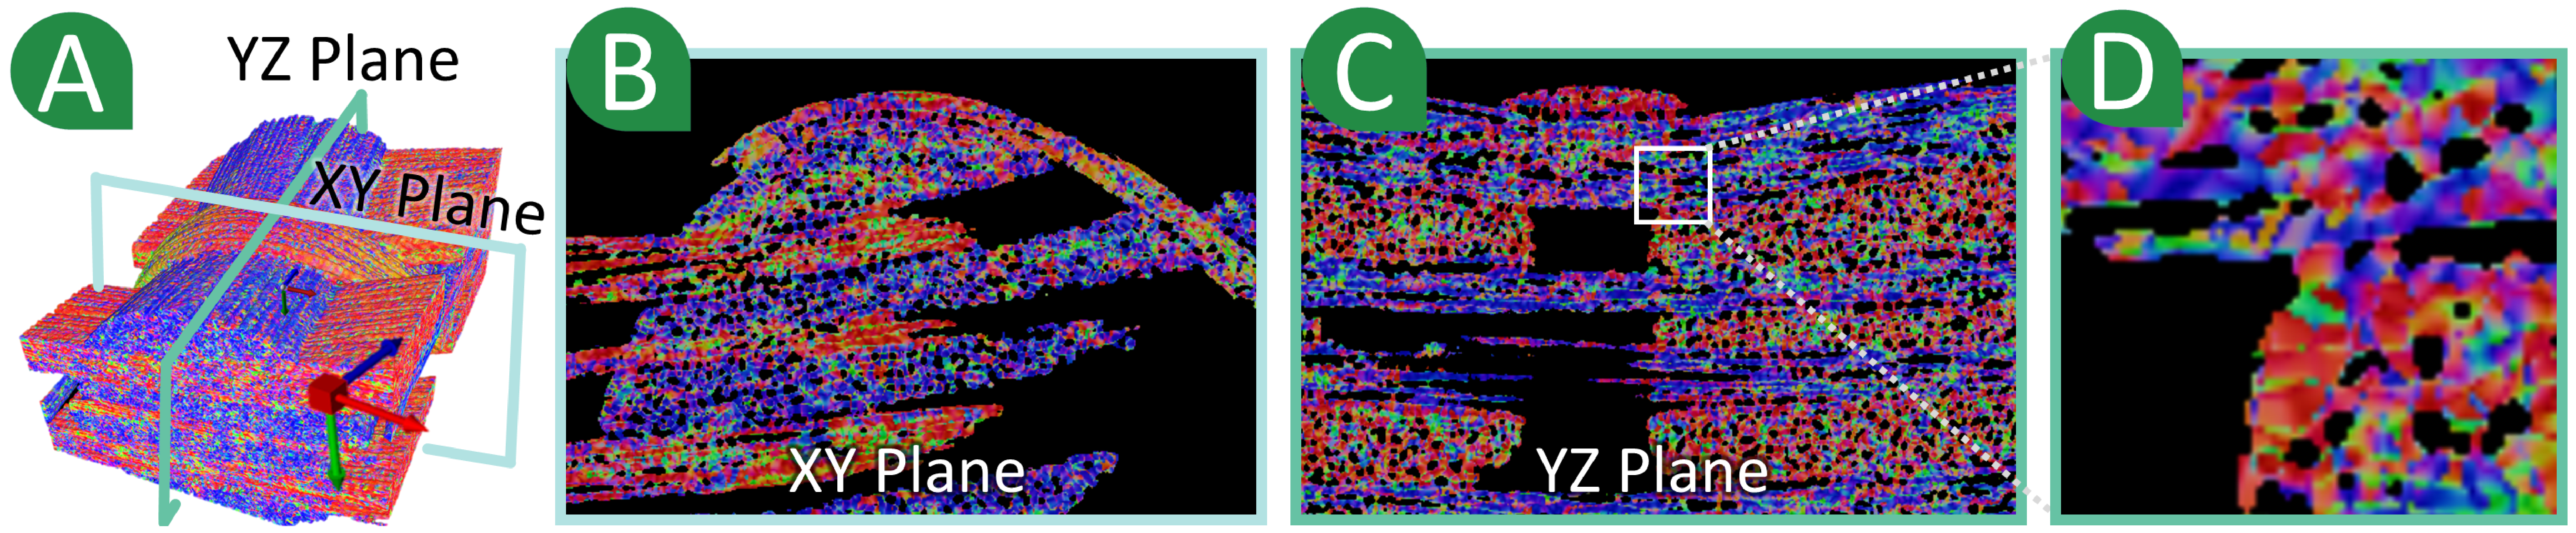
\includegraphics[width=\linewidth]{images_pvis/reliable_hessian.eps}
 \vspace{-1.5em}
\caption{Reliable Hessians. (a) Colored according to Orientation vector mapped to RGB. (b\added{,c}) 2D slice\added{s} along Z\replacedWith{ and (c) along}{-} and X axis. (d) \replacedWith{Magnified}{Zoom in of the white} region marked in \replacedWith{green square}{(c)}.}
\label{fig:reliable_hessian}
\vskip-0.2cm
\end{figure}

Figure~\ref{fig:reliable_hessian}  shows the intermidiate results of local orientation computation.
The unit vector representing the principal direction has been mapped to RGB color space.


 only at locations where $R_{H}$ is greater than the cutoff threshold. The unit vector representing the principal direction has been mapped to RGB color space. Figure~\ref{fig:reliable_hessian}a shows the entire data set. %Regions where the principal direction is parallel to the X axis are red in color, directions parallel to Y are green and those parallel to the Z are blue. 
Figure~\ref{fig:reliable_hessian}b,c show 2D slices along the Z and X axes respectively. Figure~\ref{fig:reliable_hessian}d shows a magnified region of interest. Note, the dark regions within bundles are regions where the $R_H$ is less than the threshold and are unreliable. The bundles are not uniformly colored and the Hessians and the corresponding directions are noisy.

\subsection{\mt Properties}\label{subsec:mt_properties}
\subsection{\mt Generation}\label{subsec:mt_generation}
